\documentclass{ctexart}
\ctexset{
	section={
		name={,、},
		number=\chinese{section},
		aftername={\hspace{0pt}},
	}
}
\setCJKmainfont[Mapping = fullwidth-stop]{SourceHanSerifCN-Regular}
\usepackage[a4paper,left=2cm,right=2cm,top=2.5cm,bottom=2.5cm]{geometry}
\def\theenumi{\arabic{enumi}}
\def\labelenumi{(\theenumi)}
\setlength{\headheight}{13pt}
\usepackage{fancyhdr}
\pagestyle{fancy}
\fancyhf{}
\fancyhead[C]{江理学习资料库:\mbox{\url{https://github.com/sikouhjw/jxust-Learning-database}}}
\fancyfoot[C]{\thepage}
\usepackage{amsmath,upgreek}
\let\lvert\relax\let\rvert\relax\let\lVert\relax\let\rVert\relax
\usepackage{newtxmath}
\usepackage{siunitx,physics}
\usepackage{tabularx}
\newcolumntype{Y}{>{\centering\arraybackslash}X}
\usepackage{theorem}
{
	\theoremstyle{change}
	\theoremheaderfont{\bfseries}
	\theorembodyfont{\normalfont}
	\newtheorem{ti}{}[section]
}
\usepackage{tikz}
\usetikzlibrary{shapes.geometric,calc,arrows.meta}
\usepackage[bookmarksopen = true,bookmarksnumbered = true]{hyperref}
\newcommand*{\circled}[1]{\lower.7ex\hbox{\tikz\draw (0pt, 0pt)%
	circle (.5em) node {\makebox[1em][c]{\small #1}};}}
\renewcommand{\theti}{\arabic{ti}.}
\def\hua{\mbox{\uline{\hspace{2.5cm}}}}
\def\ee{\mathrm{e}}
\def\jj{\mathrm{j}}
\title{《数字信号处理》自测题}
\author{秦舒雅}
\begin{document}
\maketitle
\section{填空题(每空 2 分,共 40 分)}
\begin{ti}
	已知 A/D 转换器的抽样周期 $T = \SI{0.1}{s}$,那么要使得信号可以复原,模拟信号的最高截止频率为 \hua (\si{s});如果以该抽样周期得到的数字信号的数字频率为 $\uppi$,那么对应的模拟信号的频率是 \hua (\si{Hz})。
\end{ti}

\begin{ti}
	虚信号满足 $x(-n) = - x(n)$,那么其傅里叶变换 $X(\ee^{\jj \omega})$ 的虚部等于 \hua 。
\end{ti}

\begin{ti}
	信号 $x(n) = 7 \sin \bigl( \frac{5}{4n} + \frac{\uppi}{2} \bigr)$ \hua (填周期或非周期)信号。如果是周期信号,则最小周期是 \hua (非周期信号请填没有)。
\end{ti}

\begin{ti}
	第一类线性相位 FIR 滤波器的 $h(n)$ 应满足 \hua ;第二类线性相位 FIR 滤波器的 $h(n)$ 应满足 \hua 。
\end{ti}

\begin{ti}
	信号 $x(n) = \{ 1,\uline{1},5,2 \}$ 的能量是 \hua 。左序列 \hua (填“是”或“否”)为反因果信号。
\end{ti}

\begin{ti}
	信号 $x(n) = \{ \uline{5},7,11 \}$ 用单位脉冲信号及其加权为 $x(n) = $ \hua 。
\end{ti}

\begin{ti}
	系统的输入输出满足 $y(n) = T[x(n)] = \sum_{k = -\infty}^{n} 3 x(k)$,那么系统是 \hua (填因果与非因果)系统,\hua (填稳定与不稳定)系统。
\end{ti}

\begin{ti}
	已知因果信号 $h(n)$ 的共轭对称部分 $h_{e}(n) = \{ 3,2,\uline{3},2,3 \}$,那么 $h(n) = $ \hua 。
\end{ti}

\begin{ti}
	$\bigl( \frac{1}{11} \bigr)^{n} u(n)$ 的 $z$ 变换为 \hua 。
\end{ti}

\begin{ti}
	已知一个因果系统 $h(n)$ 如图~\ref{fig:1} 所示,若需要设计 FIR 滤波器,其阶数 $N = $ \hua ;延迟 $\tau = $ \hua 。
	\begin{figure}[htbp]
		\centering
		\begin{tikzpicture}
			\draw[-latex] (-1,0) -- (4.5,0) node[below] {$n$};
			\draw[-latex] (0,-2) -- (0,2) node[right] {$h(n)$};
			\node[xshift = -0.2cm,yshift = -0.2 cm] {$0$};
			\node[below] at (1,0) {2};
			\node[below] at (2,0) {4};
			\node[above] at (3,0) {6};
			\node[above] at (4,0) {8};
			\filldraw (0,0.5) circle (0.05);
			\filldraw (0.5,1) circle (0.05);
			\filldraw (1,1.5) circle (0.05);
			\filldraw (1.5,1.5) circle (0.05);
			\filldraw (2,1) circle (0.05);
			\filldraw (2.5,0.5) circle (0.05);
			\filldraw (3,-0.5) circle (0.05);
			\filldraw (3.5,-1) circle (0.05);
			\filldraw (4,-0.5) circle (0.05);
			\draw (0.5,0) -- ++ (0,1);
			\draw (1,0) -- ++ (0,1.5);
			\draw (1.5,0) -- ++ (0,1.5);
			\draw (2,0) -- ++ (0,1);
			\draw (2.5,0) -- ++ (0,0.5);
			\draw (3,0) -- ++ (0,-0.5);
			\draw (3.5,0) -- ++ (0,-1);
			\draw (4,0) -- ++ (0,-0.5);
			\draw[dashed] (0,1.5) -- (1.5,1.5);
			\draw[dashed] (0,1) -- (2,1);
			\draw[dashed] (0,0.5) -- (2.5,0.5);
			\draw[dashed] (0,-0.5) -- (3,-0.5);
		\end{tikzpicture}
		\caption{}\label{fig:1}
	\end{figure}
\end{ti}

\begin{ti}
	$x_{1}(n) = \{ \uline{2},3,7,1 \}$,$x_{2}(n) = \{ \uline{1},4,3,2 \}$,则 $x_{1}(n) \circled{4} x_{2}(n) = $ \hua 。当 $L = $ \hua 时,$x_{1}(n),x_{2}(n)$ 的循环卷积与其卷积相等。
\end{ti}

\begin{ti}
	系统的输入输出满足 $y(n) = T[x(n)] = 5 x(n) + 3$,那么系统是 \hua (填线性与非线性)系统,\hua (填时变与时不变)系统。
\end{ti}

\section{(15 分)}
图~\ref{fig:2} 为 8 点 DIT-{}-FFT 的示意图,输入 $x(n) = \{ 0,1,0,1,0,1,0,1 \}$,请填写 (1)-(18) 的数字,并将答案填入相对应表格的空里。(可不写计算过程)
\begin{figure}[htbp]
	\centering
	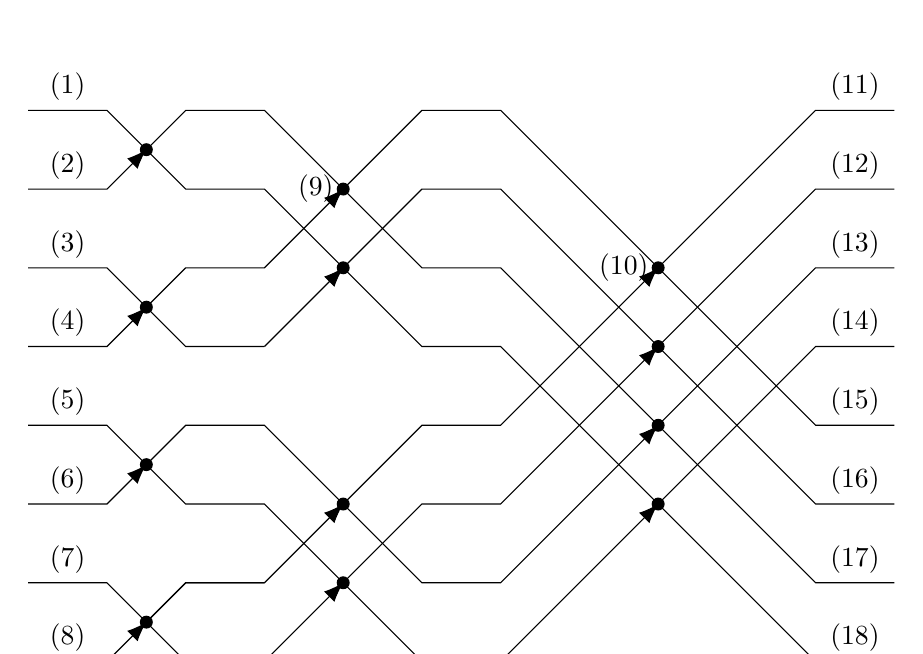
\begin{tikzpicture}
		\draw (0,0) -- node[above] {(1)} ++ (1,0) -- ++ (-45:{sqrt(2)}) -- ++ (1,0) -- ++ (-45:{2*sqrt(2)}) -- ++ (1,0) -- ++ (-45:{4*sqrt(2)}) -- node[above] {(18)} ++ (1,0);
		\draw[-{Latex[length=2.5mm]}] (0,-1) -- node[above] {(2)} ++ (1,0) -- ++ (45:{sqrt(2)/2});
		\draw (0,-1) ++ (1,0) ++ (45:{sqrt(2)/2}) -- ++ (45:{sqrt(2)/2}) -- ++ (1,0) -- ++ (-45:{2*sqrt(2)}) -- ++ (1,0) -- ++ (-45:{4*sqrt(2)}) -- node[above] {(17)} ++ (1,0);
		\draw (0,-2) -- node[above] {(3)} ++ (1,0) -- ++ (-45:{sqrt(2)}) -- ++ (1,0);
		\draw[-{Latex[length=2.5mm]}] (0,-2) ++ (1,0) ++ (-45:{sqrt(2)}) ++ (1,0) -- ++ (45:{sqrt(2)});
		\draw (0,-2) ++ (1,0) ++ (-45:{sqrt(2)}) ++ (1,0) ++ (45:{sqrt(2)}) -- ++ (45:{sqrt(2)}) -- ++ (1,0) -- ++ (-45:{4*sqrt(2)}) -- node[above] {(16)} ++ (1,0);
		\draw[-{Latex[length=2.5mm]}] (0,-3) -- node[above] {(4)} ++ (1,0) -- ++ (45:{sqrt(2)/2});
		\draw[-{Latex[length=2.5mm]}] (0,-3) ++ (1,0) ++ (45:{sqrt(2)/2}) -- ++ (45:{sqrt(2)/2}) -- ++ (1,0) -- ++ (45:{sqrt(2)}) node[left] {(9)};
		\draw (0,-3) ++ (1,0) ++ (45:{sqrt(2)/2}) ++ (45:{sqrt(2)/2}) ++ (1,0) ++ (45:{sqrt(2)}) -- ++ (45:{sqrt(2)}) -- ++ (1,0) -- ++ (-45:{4*sqrt(2)}) -- node[above] {(15)} ++ (1,0);
		\draw[-{Latex[length=2.5mm]}] (0,-4) -- node[above] {(5)} ++ (1,0) -- ++ (-45:{sqrt(2)}) -- ++ (1,0) -- ++ (-45:{2*sqrt(2)}) -- ++ (1,0) -- ++ (45:{2*sqrt(2)});
		\draw (0,-4) ++ (1,0) ++ (-45:{sqrt(2)}) ++ (1,0) ++ (-45:{2*sqrt(2)}) ++ (1,0) ++ (45:{2*sqrt(2)}) -- ++ (45:{2*sqrt(2)}) -- node[above] {(14)} ++ (1,0);
		\draw[-{Latex[length=2.5mm]}] (0,-5) -- node[above] {(6)} ++ (1,0) -- ++ (45:{sqrt(2)/2});
		\draw[-{Latex[length=2.5mm]}] (0,-5) ++ (1,0) ++ (45:{sqrt(2)/2}) -- ++ (45:{sqrt(2)/2}) -- ++ (1,0) -- ++ (-45:{2*sqrt(2)}) -- ++ (1,0) -- ++ (45:{2*sqrt(2)});
		\draw (0,-5) ++ (1,0) ++ (45:{sqrt(2)/2}) ++ (45:{sqrt(2)/2}) ++ (1,0) ++ (-45:{2*sqrt(2)}) ++ (1,0) ++ (45:{2*sqrt(2)}) -- ++ (45:{2*sqrt(2)}) -- node[above] {(13)} ++ (1,0);
		\draw[-{Latex[length=2.5mm]}] (0,-6) -- node[above] {(7)} ++ (1,0) -- ++ (-45:{sqrt(2)}) -- ++ (1,0) -- ++ (45:{sqrt(2)});
		\draw[-{Latex[length=2.5mm]}] (0,-6) ++ (1,0) ++ (-45:{sqrt(2)}) ++ (1,0) ++ (45:{sqrt(2)}) -- ++ (45:{sqrt(2)}) -- ++ (1,0) -- ++ (45:{2*sqrt(2)});
		\draw (0,-6) ++ (1,0) ++ (-45:{sqrt(2)}) ++ (1,0) ++ (45:{sqrt(2)}) ++ (45:{sqrt(2)}) ++ (1,0) ++ (45:{2*sqrt(2)}) -- ++ (45:{2*sqrt(2)}) -- node[above] {(12)} ++ (1,0);
		\draw[-{Latex[length=2.5mm]}] (0,-7) -- node[above] {(8)} ++ (1,0) -- ++ (45:{sqrt(2)/2});
		\draw[-{Latex[length=2.5mm]}] (0,-7) ++ (1,0) ++ (45:{sqrt(2)/2}) -- ++ (45:{sqrt(2)/2}) -- ++ (1,0) -- ++ (45:{sqrt(2)});
		\draw[-{Latex[length=2.5mm]}] (0,-7) ++ (1,0) ++ (45:{sqrt(2)/2}) -- ++ (45:{sqrt(2)/2}) -- ++ (1,0) ++ (45:{sqrt(2)}) -- ++ (45:{sqrt(2)}) -- ++ (1,0) -- ++ (45:{2*sqrt(2)}) node[left] {(10)};
		\draw (0,-7) ++ (1,0) ++ (45:{sqrt(2)}) ++ (1,0) ++ (45:{sqrt(2)}) ++ (45:{sqrt(2)}) ++ (1,0) ++ (45:{2*sqrt(2)}) -- ++ (45:{2*sqrt(2)}) -- node[above] {(11)} ++ (1,0);
		\filldraw (0,0) ++ (1,0) ++ (-45:{sqrt(2)/2}) circle (0.075);
		\filldraw (0,0) ++ (1,0) ++ (-45:{sqrt(2)/2}) ++ (0,-2) circle (0.075);
		\filldraw (0,0) ++ (1,0) ++ (-45:{sqrt(2)/2}) ++ (0,-4) circle (0.075);
		\filldraw (0,0) ++ (1,0) ++ (-45:{sqrt(2)/2}) ++ (0,-6) circle (0.075);
		\filldraw (0,0) ++ (3,0) ++ (-45:{sqrt(2)}) circle (0.075);
		\filldraw (0,0) ++ (3,0) ++ (-45:{sqrt(2)}) ++ (0,-1) circle (0.075);
		\filldraw (0,0) ++ (3,0) ++ (-45:{sqrt(2)}) ++ (0,-4) circle (0.075);
		\filldraw (0,0) ++ (3,0) ++ (-45:{sqrt(2)}) ++ (0,-5) circle (0.075);
		\filldraw (0,0) ++ (6,0) ++ (-45:{2*sqrt(2)}) circle (0.075);
		\filldraw (0,0) ++ (6,0) ++ (-45:{2*sqrt(2)}) ++ (0,-1) circle (0.075);
		\filldraw (0,0) ++ (6,0) ++ (-45:{2*sqrt(2)}) ++ (0,-2) circle (0.075);
		\filldraw (0,0) ++ (6,0) ++ (-45:{2*sqrt(2)}) ++ (0,-3) circle (0.075);
	\end{tikzpicture}
	\caption{}\label{fig:2}
\end{figure}
\begin{center}
	\begin{tabularx}{\textwidth}{*{9}{|Y}|}
		\hline
		1 & 2 & 3 & 4 & 5 & 6 & 7 & 8 & 9 \\
		\hline
		&&&&&&&& \\
		\hline
		10 & 11 & 12 & 13 & 14 & 15 & 16 & 17 & 18 \\
		\hline
		&&&&&&&& \\
		\hline
	\end{tabularx}
\end{center}

\section{(15 分)}
设计一个巴特沃斯高通滤波器,要求通带截止频率 $f_{\mathrm{p}} = \SI{24}{kHz}$,通带最大衰减 $a_{\mathrm{p}} = \SI{3}{dB}$,阻带截止频率 $f_{\mathrm{s}} = \SI{8}{kHz}$,阻带最小衰减 $a_{\mathrm{s}} = \SI{25}{dB}$。求出滤波器阶数以及实际滤波器的 $H_{\mathrm{a}}(s)$。已知:巴特沃斯归一化函数 $G(p) = \frac{1}{B(p)}$,
\[
	B(p) = \begin{cases}
		p + 1, & N = 1 \\
		p^{2} + 1.414 p + 1, & N = 2 \\
		(p + 1)\bigl(p^{2} + p + 1\bigr), & N = 3 \\
		\cdots\cdots
	\end{cases}
\]

\section{讨论(15 分)}
有一线性非时变系统,其系统函数为:
\[
	H(z) = \frac{1}{(1 - 0.5 z^{-1}) (1 - 0.8 z)},
\]
讨论系统的因果性和稳定性,并求出相应的单位取样响应 $h(n)$。

\section{(15 分)}
某一线性时不变因果系统满足以下条件:
\begin{enumerate}
	\item 输入信号 $x_{1}(n) = 6^{n}$,系统的零状态响应为零;
	\item 输入信号 $x_{2}(n) = u(n)$,系统的零状态响应 $y_{2}(n) = n u(n) + \alpha u(n)$。
\end{enumerate}
求系统的单位响应 $h(n)$ 及 $\alpha$。
\end{document}